\documentclass[11pt]{article}
\usepackage[letterpaper,margin=0.9in]{geometry}
\usepackage[hidelinks]{hyperref}
\usepackage{enumitem}
\usepackage{titlesec}
\usepackage{tabularx}
\usepackage{graphicx}

\setlist[itemize]{leftmargin=1.2em,itemsep=3pt,topsep=3pt}
\titleformat{\section}{\large\bfseries}{}{0em}{}[\titlerule]

\newcommand{\entry}[4]{
  \noindent\begin{tabularx}{\textwidth}{@{}Xr@{}}
    \textbf{#1} & #2 \\
    \textit{#3} & \textit{#4}
  \end{tabularx}\vspace{2pt}
}

\begin{document}

\noindent\begin{minipage}[t]{0.76\textwidth}
\vspace{0pt}
{\LARGE \textbf{Piter Z. Garcia Bautista}}\\[4pt]
Rochester, NY \textbar\ +1 (646) 288-3300 \textbar\ \href{mailto:pzg8794@rit.edu}{pzg8794@rit.edu}\\
\href{https://linkedin.com/in/garciapiterz}{linkedin.com/in/garciapiterz} \textbar\
\href{https://github.com/pzg8794}{github.com/pzg8794} \textbar\
\href{https://garciapiterz.com}{garciapiterz.com}
\end{minipage}%
\hfill\begin{minipage}[t]{0.20\textwidth}
\vspace{0pt}
\raggedleft
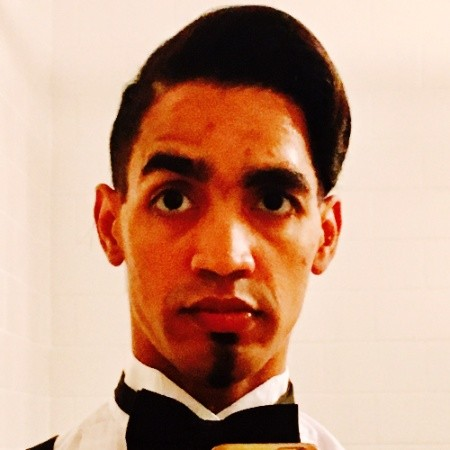
\includegraphics[width=\linewidth]{profile_pic}
\end{minipage}
\vspace{6pt}

\section{Research Profile}
Graduate researcher focused on machine learning for diagnostics and decision support under noisy, heterogeneous, and partially observed data. Background includes an M.S. in Computer Science, current M.S. work in Data Science, industry healthcare AI experience, and computational biology training. Current work emphasizes reproducibility, robust evaluation, fairness-aware analysis, and translational relevance to clinical settings.

\section{Research Interests}
Machine learning for precision medicine and diagnostics; robust learning under missing or uncertain context; fairness-aware and trustworthy AI for high-stakes decision support; reproducible computational evaluation systems.

\section{Education}
\entry{Rochester Institute of Technology}{Expected Aug 2026}{Master of Science, Data Science --- GPA 3.9}{Rochester, NY}
\begin{itemize}
  \item Concentration: Bioinformatics \& Artificial Intelligence.
  \item Relevant coursework: Bioinformatics Algorithms, Data-Driven Knowledge Discovery, Neural Networks, Applied Statistics, Software Engineering for Data Science.
\end{itemize}

\entry{University of Rochester, Warner School of Education}{In progress}{Graduate study, Teaching Computer Science K--12 (M.S. track) --- GPA 4.0}{Rochester, NY}
\begin{itemize}
  \item NSF Robert Noyce Scholar (\$30,000 full funding); Advanced Certificate in Leadership in Disability and Inclusive Practices.
\end{itemize}

\entry{Rochester Institute of Technology}{2015}{Master of Science, Computer Science --- GPA 3.2}{Rochester, NY}
\begin{itemize}
  \item Concentrations: Artificial Intelligence, Big Data Analytics, Computer Graphics.
\end{itemize}

\entry{Farmingdale State College}{2012}{Bachelor of Science, Computer Engineering Technology --- GPA 3.3}{Farmingdale, NY}
\begin{itemize}
  \item Foundations in computer hardware, embedded systems, and engineering design; early technical training for computational problem-solving.
\end{itemize}

\section{Research and Professional Experience}
\entry{Rochester Institute of Technology, Software Engineering Department}{Fall 2025 -- Present}{Graduate Assistant, Quantum and AI Research}{Rochester, NY}
\begin{itemize}
  \item Build reproducible machine learning evaluation pipelines across local, Colab, and GCP environments with structured logging and validation.
  \item Develop experimental bandit and decision-making systems for uncertain, heterogeneous settings, with emphasis on reliability and traceability.
  \item Produce manuscript-ready technical analyses and research artifacts for faculty-led projects.
\end{itemize}

\entry{University of Rochester, Warner School of Education}{Sep 2024 -- Present}{CS Teacher Candidate \& Education Research (NSF Noyce Scholar)}{Rochester, NY}
\begin{itemize}
  \item Deliver K--12 computer science instruction in active public school placement as part of the NSF Robert Noyce Scholar program, including computational thinking, inclusive pedagogy, and NYS learning standards.
  \item Conduct applied education research on AI-informed and data-driven approaches to improve learning outcomes for neurodivergent students, applying Universal Design for Learning (UDL) and evidence-based adaptive strategies.
  \item Produce lesson artifacts and instructional analyses documenting the intersection of AI, inclusive education, and evidence-based CS pedagogy.
\end{itemize}

\entry{Rochester Institute of Technology}{2026}{Computational Biology Research Projects (BIO614 and BIO550)}{Rochester, NY}
\begin{itemize}
  \item Led substantial computational work in BIO614, including formal manuscript development in the project \textit{BIO614-FinalProjectProposal} (Overleaf), emphasizing algorithm implementation, structured evaluation, and scientific reporting.
  \item Complemented BIO614 with BIO550 RNA-seq and differential-expression analysis, including reproducible preprocessing, quality-control validation, and biological interpretation.
\end{itemize}

\entry{VEDADATA Inc.}{Sep 2022 -- Aug 2024}{Data Solutions Engineer}{New York, NY}
\begin{itemize}
  \item Designed scalable Python and pandas workflows for ingestion, validation, preprocessing, and analytics operations.
  \item Strengthened production data reliability through structured quality checks and statistical diagnostics.
\end{itemize}

\entry{VIOME Inc.}{Jan 2021 -- Sep 2022}{AI Data Solutions Engineer}{New York, NY}
\begin{itemize}
  \item Developed healthcare-oriented machine learning workflows for preprocessing, feature engineering, model experimentation, and evaluation.
  \item Supported reproducible analytics workflows in AWS-based environments for predictive health applications.
\end{itemize}

\section{Selected Technical Writing}
\begin{itemize}
  \item \textit{Big Data Medical Diagnosis: A Multi-Method Approach} (RIT M.S.\ Computer Science graduate research, 2015) --- ensemble and deep learning methods for clinical classification on high-dimensional biomedical data.
  \item \textit{Predicting Hospital Readmission Rates: A Multi-Method ML Analysis} (DSCI-633 Project Report, 2025) --- ensemble and regularized regression methods for clinical risk stratification under distribution shift.
  \item \textit{BIO614-FinalProjectProposal} (Overleaf manuscript, 2026) --- RNA secondary structure prediction with thermodynamic deep learning enhancements, reproducible benchmarking, and biological interpretation.
  \item \textit{Equitable Bioinformatics: Enhancing Diagnostic Decision-Making through RNA and Biomarker Data} (ISTE-780 Project Report, 2025) --- fairness-aware ML for genomic diagnostic algorithms with SHAP-based bias detection and statistical significance testing.
  \item \textit{Differential Gene Expression in Murine DRG Neurons Following Sciatic Nerve Injury: An NGS Reanalysis} (BIOL550 Computational Biology Project, 2026) --- reproducible bulk RNA-seq pipeline using DESeq2, QC validation, and pathway-level biological interpretation of nociceptor gene expression.
  \item \textit{Fairness-Aware Bandits for Clinical Decision Systems} (DSCI-601 Project Proposal, 2025) --- bandit learning with equity constraints applied to high-stakes clinical diagnostic decision-making, addressing demographic disparity in sequential clinical recommendation workflows.
\end{itemize}

\section{Awards \& Recognition}
\begin{itemize}
  \item NSF Robert Noyce Teacher Scholarship (2024--2026) --- full funding for M.S.\ in Teaching Computer Science K--12.
  \item MS International Scholarship (2012--2015) --- MESCYT \& RIT, awarded for academic excellence.
  \item Honorable Mention Technology Award (2012) --- NYS STEP/CSTEP, 2nd place capstone project.
  \item IEEE Alumni Member (2009--Present) --- Member No.\ 90613000.
\end{itemize}

\section{Technical Competencies}
\textbf{Programming:} Python, R, Java, C++, C\#, SQL, MATLAB, JavaScript, Bash\\
\textbf{Machine Learning:} PyTorch, TensorFlow, scikit-learn, XGBoost, model evaluation, uncertainty-aware analysis, fairness-aware ML\\
\textbf{Data and Statistics:} pandas, NumPy, SciPy, statistical modeling, reproducible benchmarking\\
\textbf{Research Tooling:} Git/GitHub, Linux, Docker, LaTeX, AWS, GCP

\section{Selected Fit for Uppsala Precision Medicine Position}
\begin{itemize}
  \item Combined computational biology background (BIO614 RNA structure prediction; BIO550 RNA-seq differential expression; ISTE-780 fairness-aware genomic diagnostics) directly matches the group's focus on machine learning for precision medicine and diagnostics.
  \item Strong Python-based deep learning and reproducibility foundation (PyTorch, TensorFlow, scikit-learn) aligned with the group's image analysis and cancer detection workflows.
  \item Research motivation to apply fairness-aware and uncertainty-aware ML methods to clinical datasets with direct translational relevance to cancer treatment prediction and biomarker discovery.
  \item Multidisciplinary profile spanning data science, computational biology, and health AI---suitable for collaboration across MIDA, Centre for Image Analysis, IGP, and SciLifeLab.
\end{itemize}

\end{document}